\appendix

\chapter{Appendix}
Appendix content goes here.
\section{Previous WBS}
This is where the Work Breakdown Structures from early development is placed here with the most recent placed earliest, as can be seen in Figures \ref{fig:WBS83} and \ref{fig:WBS13}.
\begin{figure}[p]

\setlength\fboxsep{0pt}
\setlength\fboxrule{1pt}\noindent\makebox[\textwidth]{%
 \fbox{
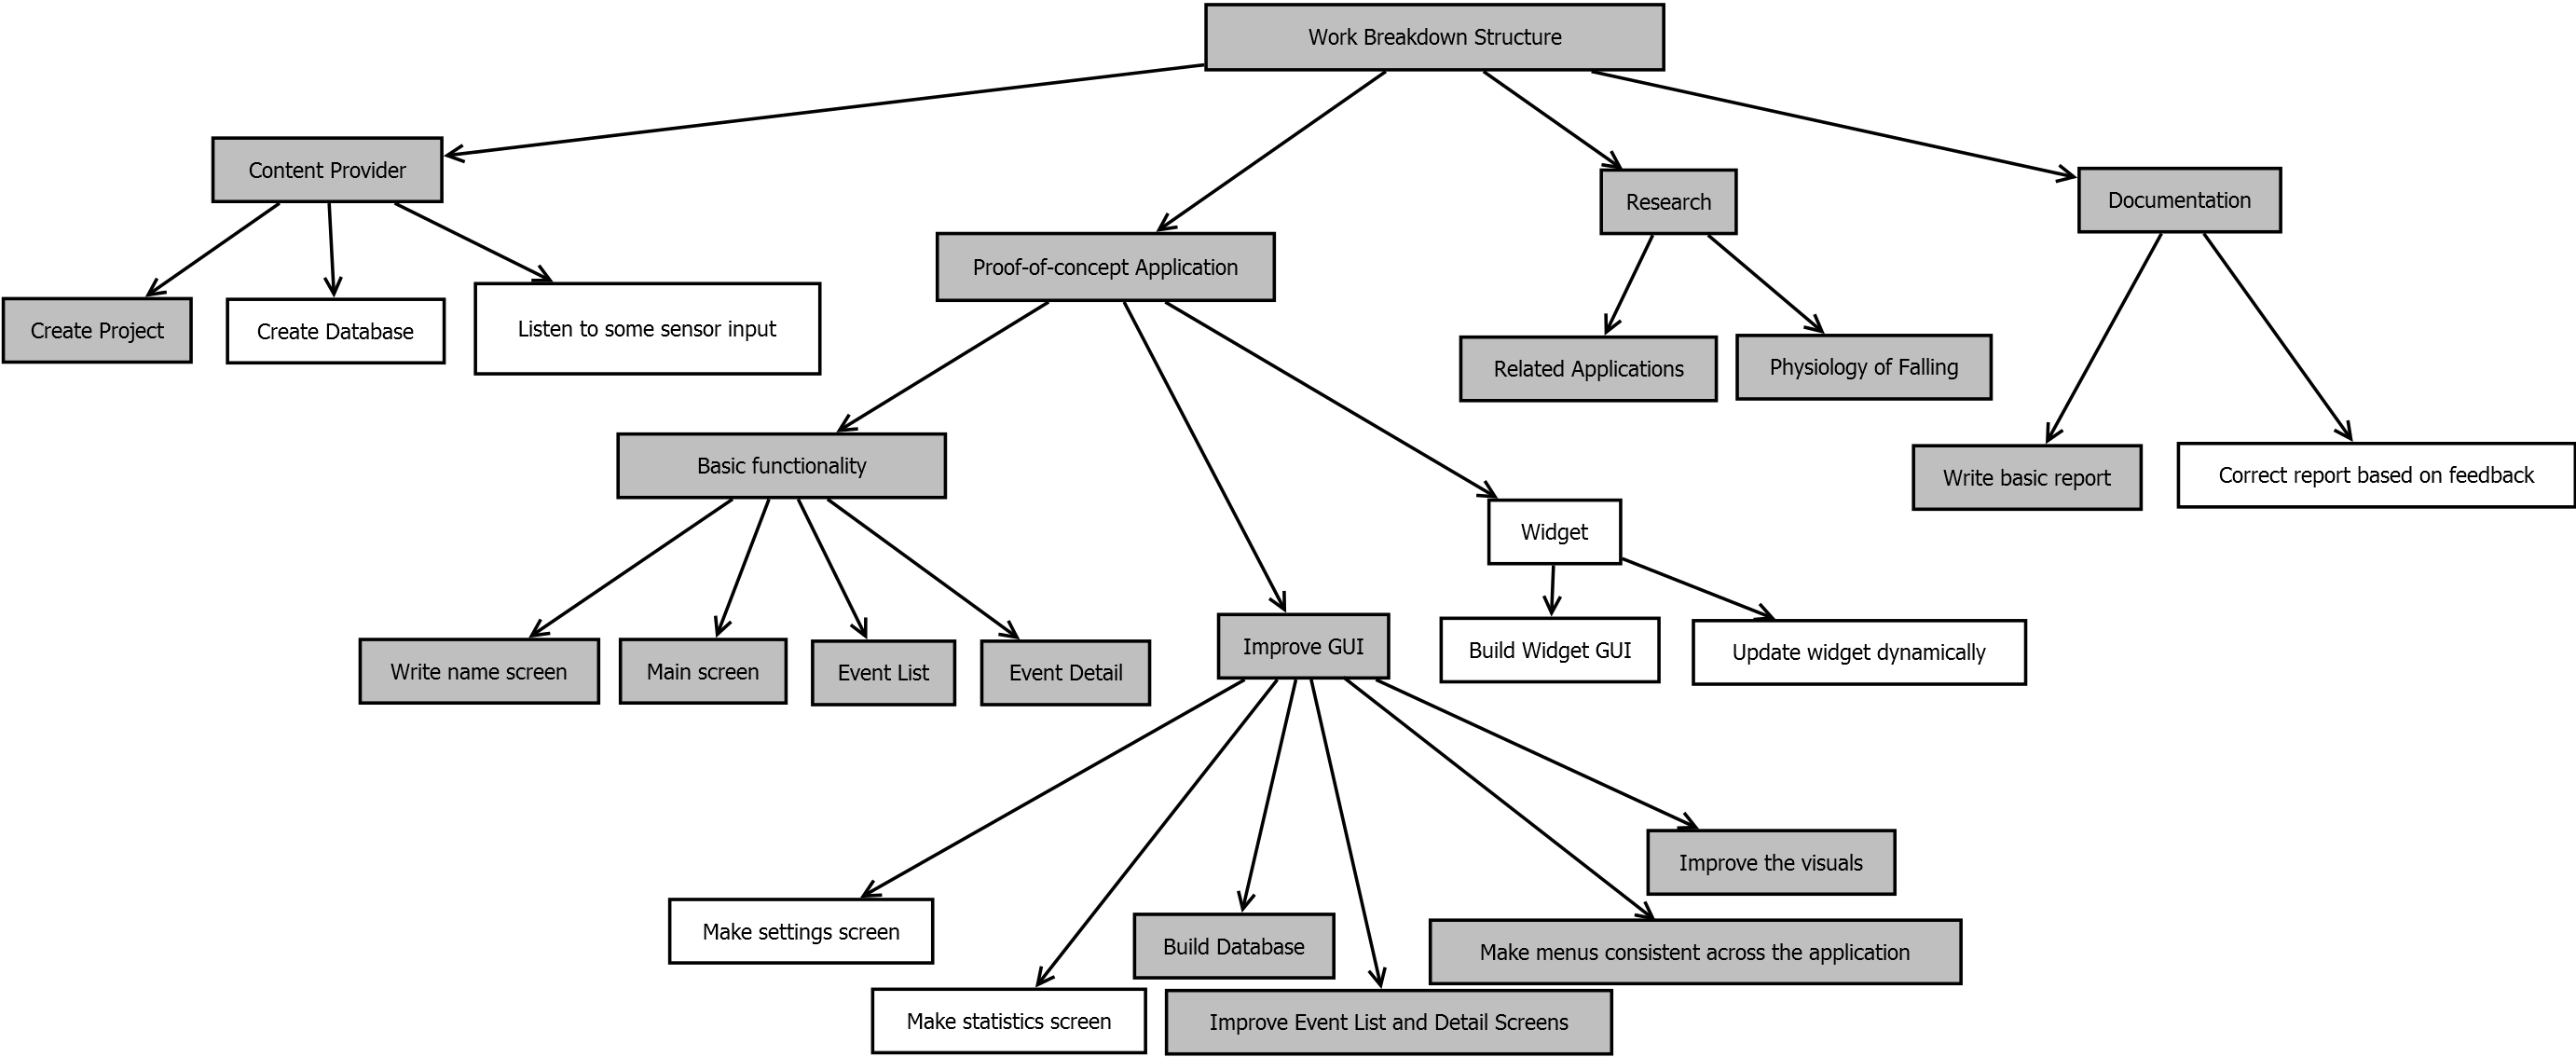
\includegraphics[width=1.45\textwidth , angle=270]{Res/WBS08313.png}
}
\label{fig:WBS83}
}

\caption{The WBS as per 8.3.13}
\end{figure}

\begin{figure}[p]

\setlength\fboxsep{0pt}
\setlength\fboxrule{1pt}\noindent\makebox[\textwidth]{%
 \fbox{
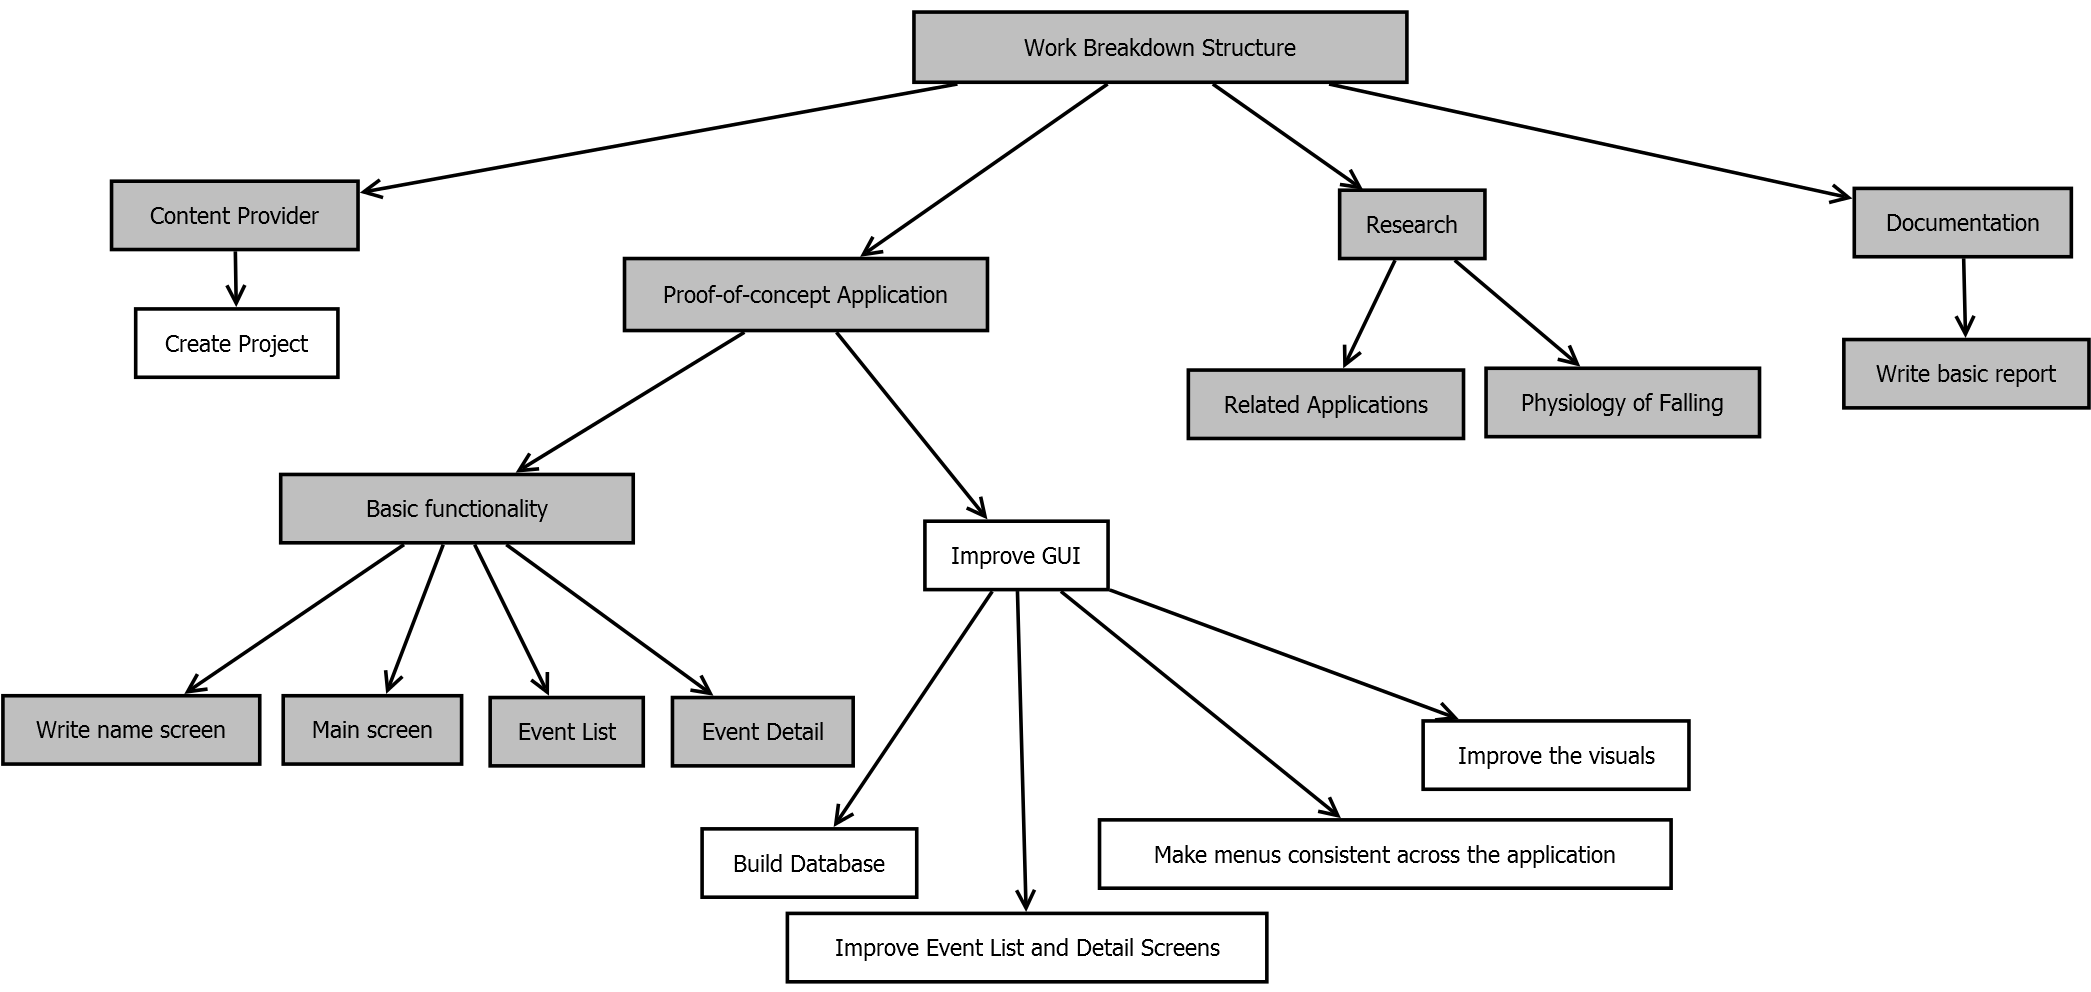
\includegraphics[width=1.45\textwidth , angle=270]{Res/WBS01313.png}
}
}
\label{fig:WBS13}
\caption{The WBS as per 1.3.13}
\end{figure}

\section{Reports}
The work done was described as short periods called sprints. 
\begin{figure}
\caption{Short summary of work done sorted by sprint}
\begin{tabular}{|c|c|p{7cm}|}
\hline
Sprint nr. & Date & Summary\\
\hline
Sprint 1: & 03.02.13 - 08.02.13 & Developing user stories and paper prototypes of the GUI.\\ 
\hline
Sprint 2: & 08.02.13 - 15.02.13 & Developing a mock-up application demonstrating the GUI.\\
\hline
Sprint 3: & 15.02.13 - 22.02.13 & Improving UI and functionality for the prototype, researching medical factors. \\
\hline
Sprint 4: & 22.02.13 - 01.03.13 & Improving secondary functionality for the prototype (settings, statistics, relatives screens),researching content-providers and alternative solutions. \\
\hline
Sprint 5: & 01.03.13 - 07.03.13 & Creating content-provider, creating presentation, finishing secondary screens (as described above), including pedometer, writing test-cases.\\
\hline
Sprint 6: & 08.03.13 - 15.03.13 &\\%TODO
\hline
Sprint 7: & 16.03.13 - 22.03.13 &todo\\%TODO
\hline
Sprint 8: & 08.03.13 - 16.03.13 &todo\\%TODO
\hline
Easter &-&little work done\\
\hline
Sprint 9: & 03.04.13 - 5.04.13 & Changing plans, removing pedometer app from project, planning new project structure\\%TODO
\hline
Sprint 10: & 6.04.13 - 12.04.13 & Creating own content-provider and step-detector, integrating all three components\\
\hline
Sprint 11: & 13.04.13 - 19.04.13 & Fixing documentation according to feedback\\
\hline 
%TODO fill this table
\end{tabular} 
\label{tab:sprintList}
\end{figure}
\newpage

\section{Apache license and notice}
\label{appendix:license}
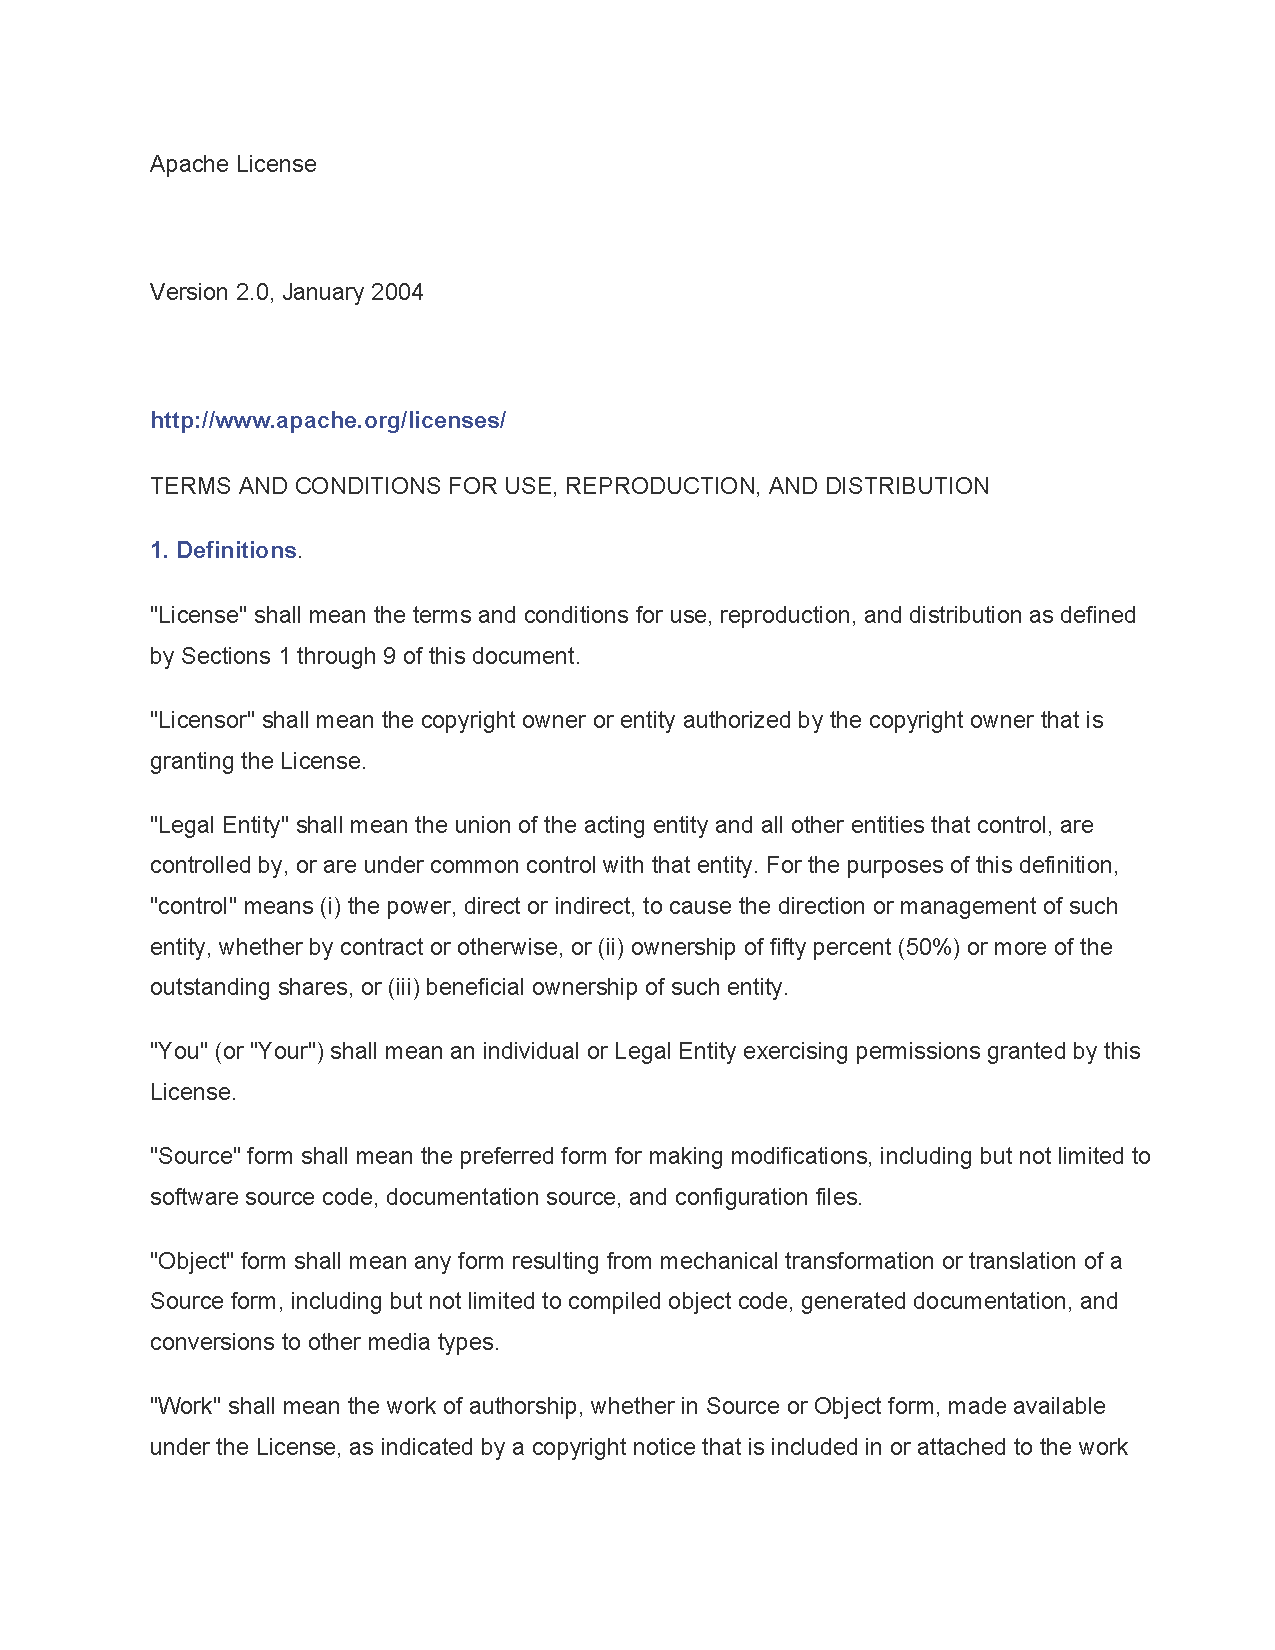
\includepdf[pages={-}]{Res/Apache2license}
\section{Meeting summaries}
Regular status reports was a part of necessary documentation. Of particular importance was reports to the supervisor, and reports done to the other group members. This status report was written during sprint 4. The reports were included in chronological order.


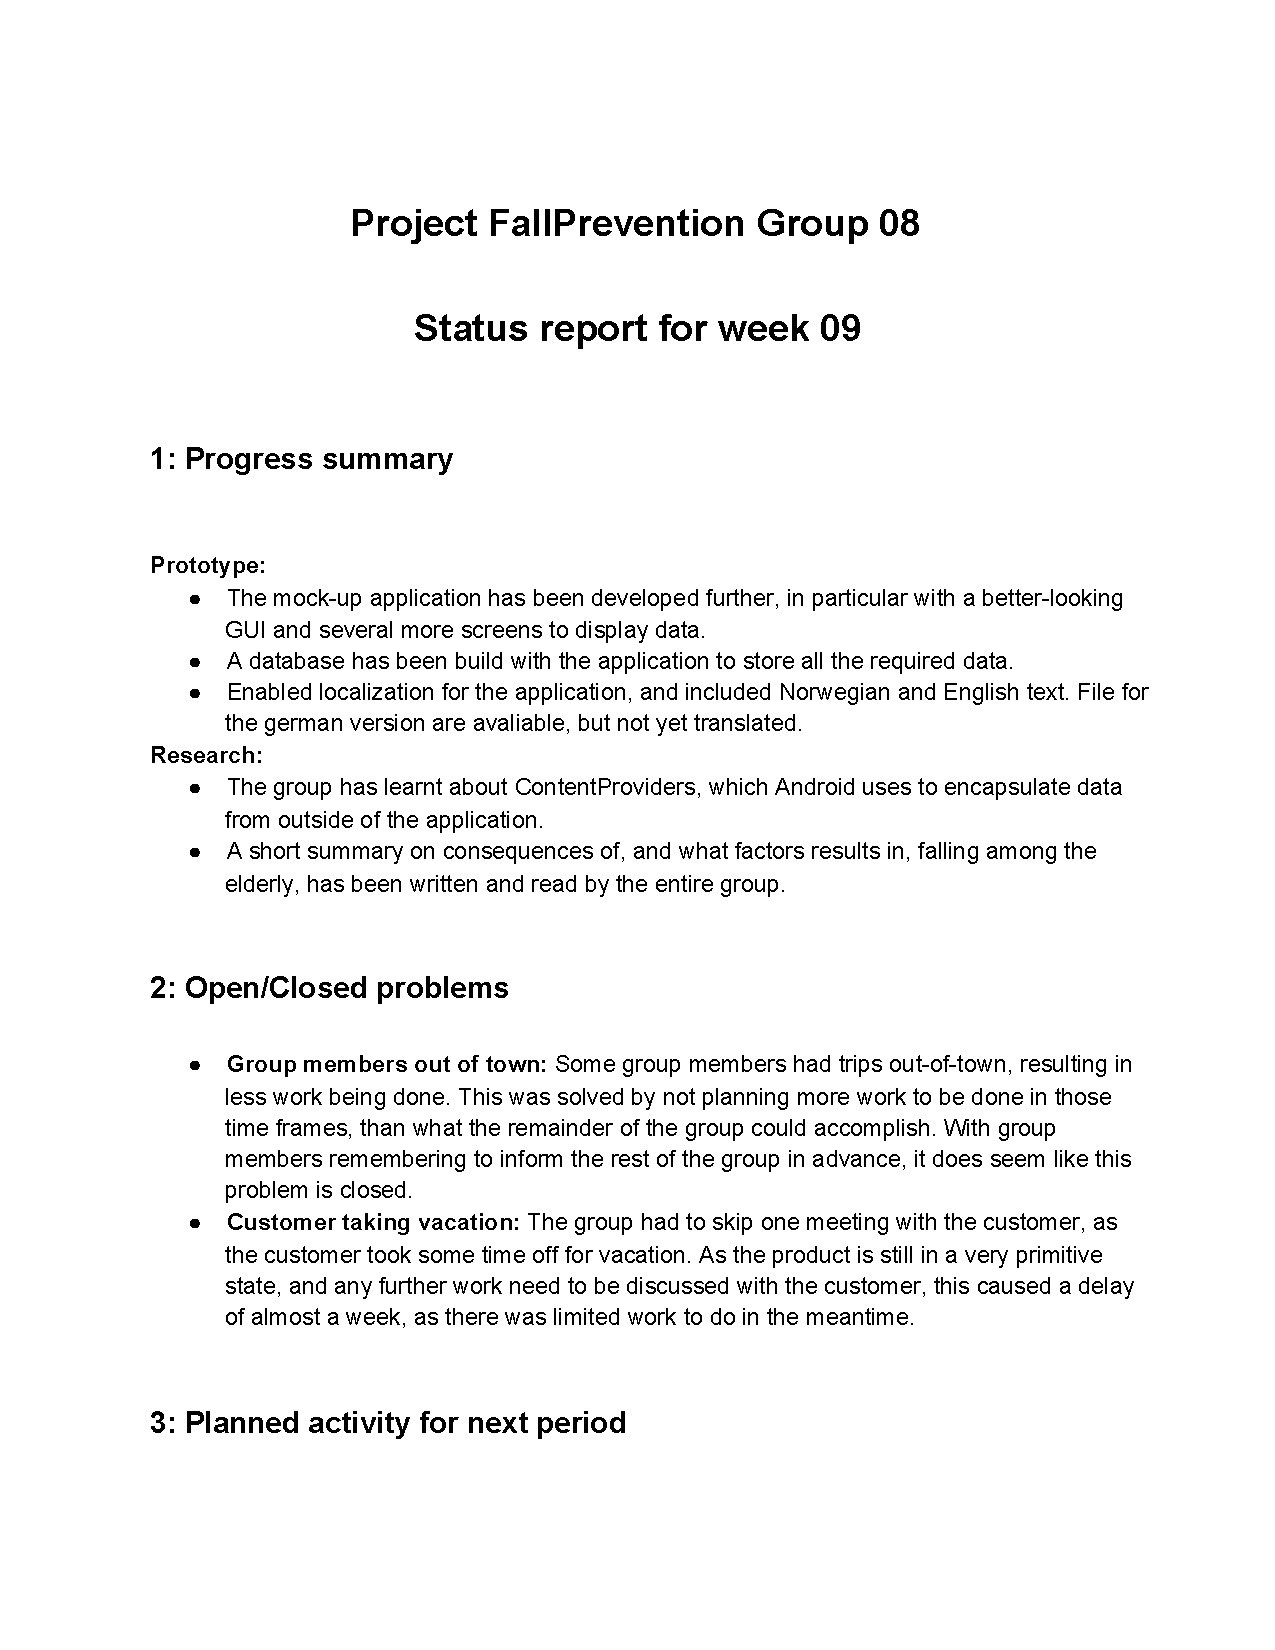
\includepdf[pages={-}]{Res/StatusReportWeek9}

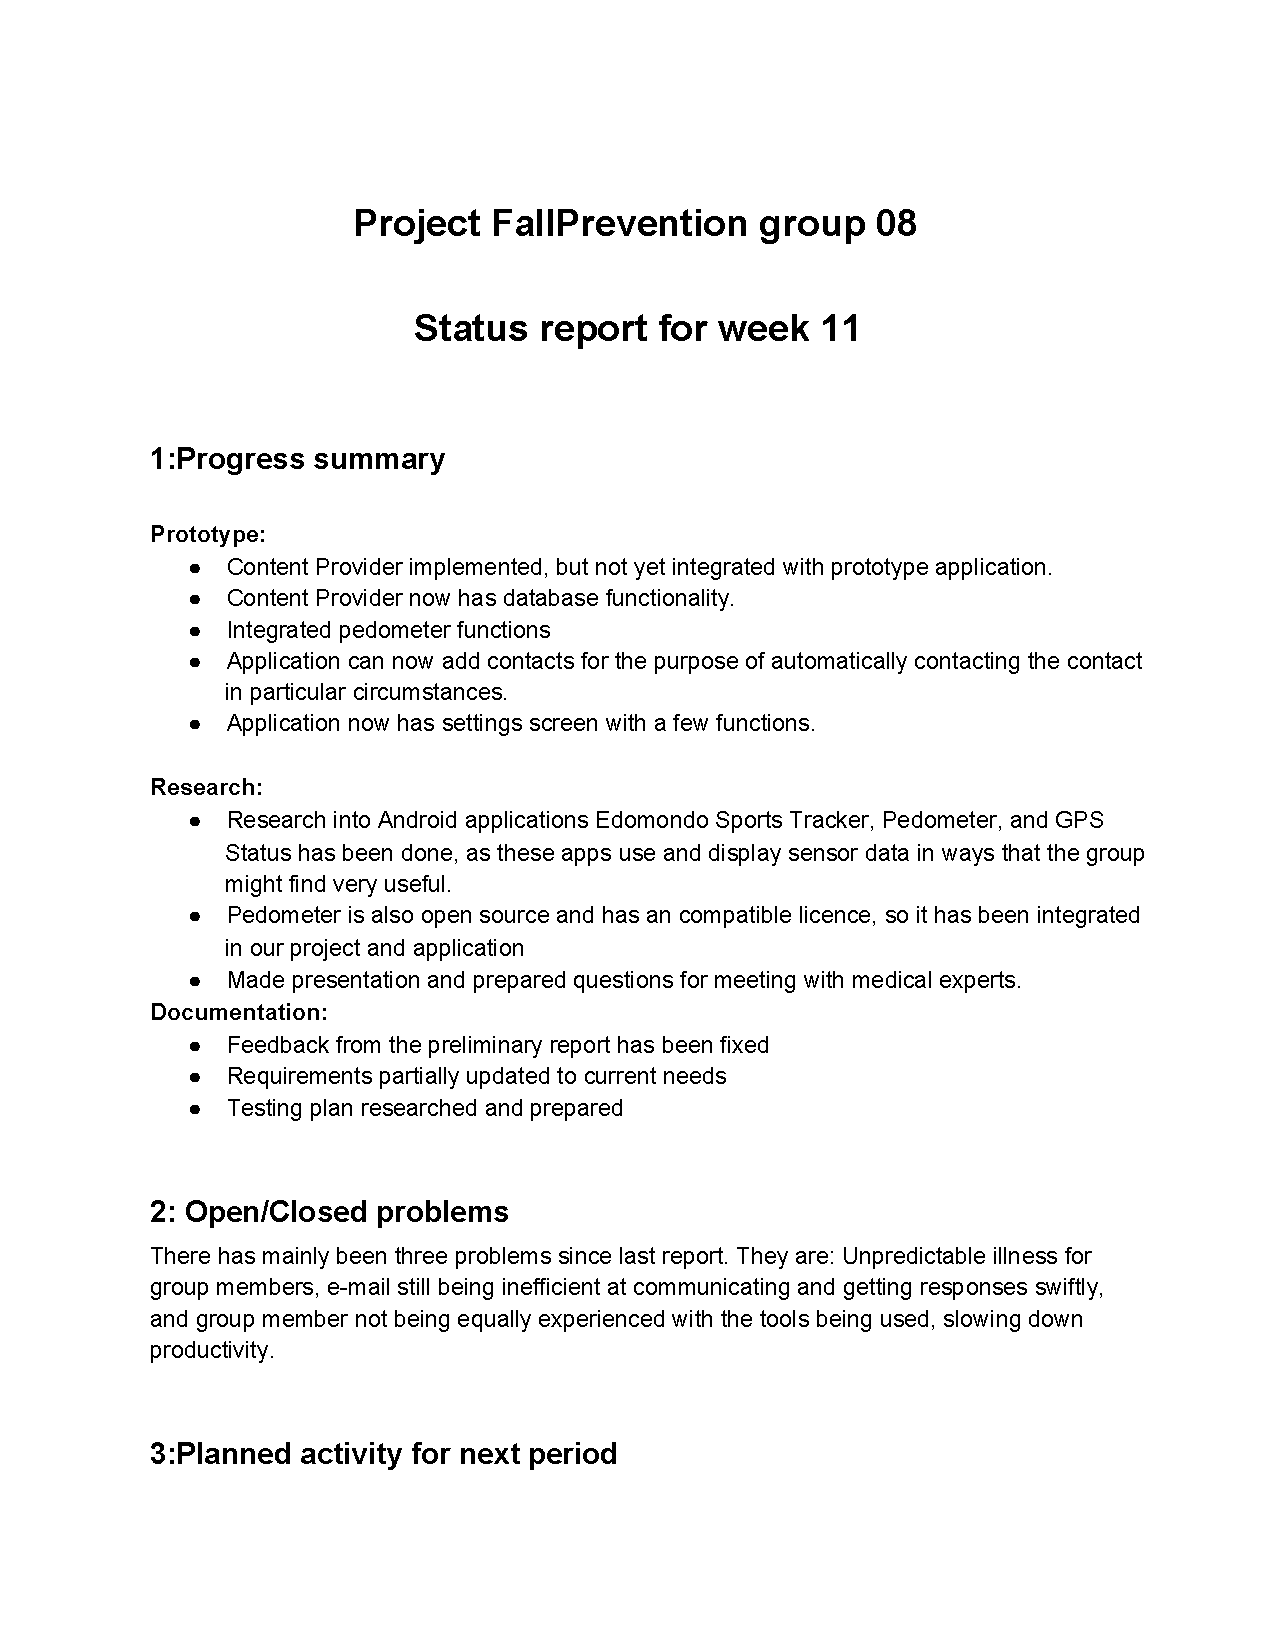
\includepdf[pages={-}]{Res/StatusReportWeek11}





